\section{Abstract}
The French 2012-2015 Commission Nationale d'Evaluation reports
\cite{cne2_reports_2015} emphasize preparation for a transition from \glspl{LWR} to \glspl{SFR}.
We used \Cyclus \cite{huff_fundamental_2016} to explore the feasibility of using \gls{UNF} from other EU nations
for French transition into a \gls{SFR} fleet without additional construction of \glspl{LWR}.
A \Cyclus simulation ran from 1950 to 2160 for EU to track the \gls{UNF} mass
and tails inventory to support
the transition into \glspl{SFR}. Another simulation ran to model French
transition to \glspl{SFR} supported by reprocessing the \gls{UNF} inventory.
These simulations demonstrate that France can avoid deployment
of additional \glspl{LWR} by accepting \gls{UNF} from other EU nations.


\section{Introduction}
We used \Cyclus to analyze
the future nuclear inventory in the European Union. \Cyclus is an agent-based extensible
framework for modeling the flow of material through future nuclear cycles .
This paper focuses on the used fuel
inventory in \gls{EU} member states in 2050, and focuses on a potential strategy of used fuel
management.
A major focus of this paper is to determine the extent to which France has an incentive
to receive all the \gls{UNF} from \gls{EU} nations to create \gls{MOX}.
The \gls{MOX} created will fuel French transition to a \gls{SFR} fleet
and allow France to avoid building additional \glspl{LWR}.

Past research, focused solely on France, typically assumes that additional \glspl{LWR},
namely \glspl{EPR} supply \gls{UNF} to produce \gls{MOX} \cite{carre_overview_2009, martin_symbiotic_2017, freynet_multiobjective_2016}.
Studies exist on implementation of partitioning and transmutation
in a regional (European) context, with \glspl{ADS} and Gen-IV reactors \cite{fazio_study_2013}.
There is little attention paid to reprocessing legacy \gls{UNF} from other
EU nations to produce \gls{MOX} for the newly deployed \glspl{SFR}.
The present work finds that this collaborative strategy can reduce the
need to construct additional \glspl{LWR} in France.

\section{Methodology}
Two \Cyclus simulations are run for this paper. 
The first simulation calculates
the mass and composition of used fuel and tails \gls{EU} nations accumulate from 1970 to 2050,
as well as the amount of \gls{MOX} that the \gls{UNF} inventory creates.
All EU nations with the exception of France adopts a once-through fuel cycle.
France can reprocess used \gls{UOX} and \gls{MOX} to
produce \gls{MOX} from reprocessed plutonium and depleted uranium (tails).

After obtaining the \gls{UNF} inventory of all \gls{EU} in 2050, the second
simulation runs where the \gls{UNF} inventory is reprocessed and fabricated
as fuel for the newly deployed \gls{SFR} reactors.
\glspl{SFR} are modeled after the ASTRID breeder reactor \cite{varaine_pre-conceptual_2012}.
The ASTRID-type \glspl{SFR} make up for the decommissioned capacity
of \glspl{LWR} in France, to remain a constant installed capacity of $66,000$ MWe up to 2160.
Eventually, the  \gls{MOX} created from recycled \gls{MOX}
fuels the entire fleet of 110 \glspl{SFR}.

All the scripts and data used
in this paper are available in \cite{bae_arfc/transition-scenarios:_2017}.

\subsection{\Cyclus}
\Cyclus is an agent-based fuel cycle simulation framework, meaning that
each reactor, reprocessing plant, and fuel fabrication plant is modeled as agents. At each timestep (one month),
agents put out their bids for materials (supply and/or demand) and exchange
with one another. This is done using a market-like mechanism called the 
dynamic resource exchange \cite{gidden_agent-based_2015}.
Each material item has a quantity, composition, name, and a unique identifier
for output analysis. 
A \Cyclus input file contains archetypes, which are fuel cycle facilities with
pre-defined parameters, that are deployed in the simulation as \texttt{facility} agents.
An \texttt{Institution} agent deploys \texttt{facility} agents
according to a user-defined deployment scheme at pre-defined timesteps.
The \texttt{Institution} agent is part of a \texttt{Region} agent,
which can contain multiple \texttt{Institution} agents.

For example, `France' would be a \texttt{Region} agent,
that may contain two \texttt{Institution} agents \glspl{LWR}
and \glspl{SFR}. The \texttt{Institution} agents would then deploy
\glspl{LWR} and \glspl{SFR} agents, respectively, according to a pre-defined deployment
scheme.


\subsection{\gls{EU} Historical Deployment Scheme}

The historical nuclear operation of \gls{EU} nations is based on
the \gls{IAEA} \gls{PRIS} database \cite{iaea_nuclear_2017}. That database is imported as a csv file, to populate the simulation
with deployment information, listing the country, reactor unit, type, net capacity (MWe), status,
operator, construction date, first criticality date, first grid date, commercial date, shutdown
date (if applicable), and unit capacity factor for 2013. Then only the \gls{EU} countries are extracted
from the csv file. We wrote up a python script to generate a \Cyclus input file from the csv file,
which lists the individual reactor units as agents. 

Projections of future reactor deployment in this simulation is based on assessment of analyses
from references such as \gls{PRIS} for reactors planned for construction \cite{iaea_nuclear_2017},
the World Nuclear Association and two other papers for future plans in EU nations
\cite{world_nuclear_association_nuclear_2017, joskow_future_2012, hatch_politics_2015}.
The projections extend to 2050 at the latest. This allows the simulation to take place from
1970 to 2050, the latest foreseeable future. Later sections explain, in detail, the specific plans for each \gls{EU} nation.

Figure \ref{fig:eu_pow} displays the
timeseries of installed capacity in \gls{EU} nations.

\begin{figure}[htbp!]
	\begin{center}
		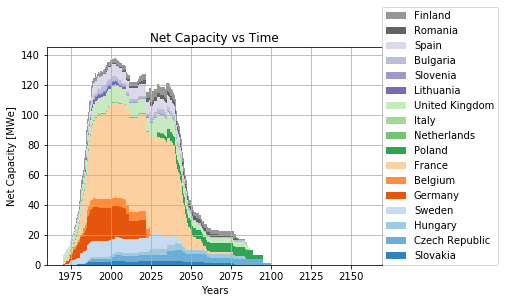
\includegraphics[scale=0.7]{./images/eu_future/power_plot.png}
	\end{center}
	\caption{The timeseries of installed nuclear capacity in the EU are separated by \texttt{Region}s in \Cyclus.
			 The sudden drops in capacity are caused by nuclear phaseout plans by nations like Germany and Belgium.
			 }
	\label{fig:eu_pow}
\end{figure}
\FloatBarrier

\subsection{French \gls{SFR} Deployment Schedule}

Once \glspl{SFR} become available in 2040,
600-MWe \glspl{SFR} are deployed to make up for the 
decommissioned \gls{LWR} capacities. 
This results in an installed capacity of 66,000 MWe
of \gls{SFR} by 2076, when the last \gls{LWR} decommissions.

\begin{figure}[htbp!]
        \begin{center}
                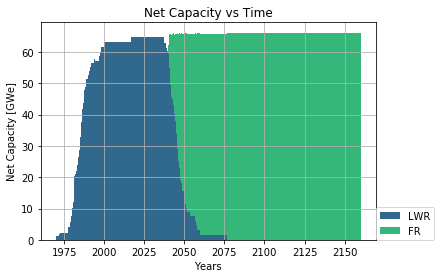
\includegraphics[scale=0.6]{./images/french-transition/power_plot.png}
        \end{center}
        \caption{This plot shows the potential French transition from \glspl{LWR} to \glspl{SFR}.
				 The aggressive growth of nuclear in the 1980s leads to a substantial shutdown
				 of nuclear in the 2040s, which would be replaced by new \glspl{SFR}. The net
				 capacity is kept at a constant of 66 GWe.}
        \label{fig:sfr_num}
\end{figure}
\begin{figure}[htbp!]
	\begin{center}
		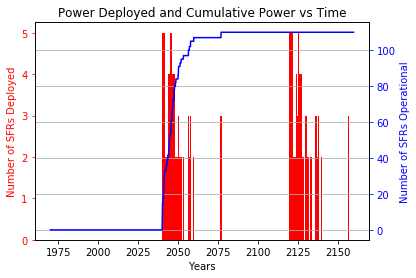
\includegraphics[scale=0.6]{./images/french-transition/sfr_deploy.png}
	\end{center}
	\caption{The deployment of \glspl{SFR} in France is characterized by a period of
		     aggressive building. An average of four reactors are built per year to
		     make up for the decommissioned power plants built in the 1980s and 1990s.
		     The second period of aggressive building occurs when the first generation
		     of \glspl{SFR} decommission after 80 years.}
	\label{fig:dep}
\end{figure}
\FloatBarrier


\Cref{fig:sfr_num} and \cref{fig:dep} display
the French transition to \glspl{SFR} over time.
The steep transition from 2040 to 2060 reflects the scheduled
decommissioning of reactors built in the 1975-2000
era of aggressive nuclear growth in France.

In reality, building five reactors every year is highly unrealistic. However,
this analysis is done to analyze material flow, claiming that, if such an aggressive
deployment scheme was to take place, the \glspl{SFR} would have enough fuel.
More realistically, the deployment of new \glspl{SFR} can be spread out by
staggering scheduled decommissioning of \glspl{LWR} through lifetime extensions.

\subsection{Material Definitions}
Depletion calculations of the nuclear fuel are recipe-based, such that a fresh 
and used fuel recipe is defined for each reactor type.
For the compositions of the fuel, a reference depletion calculation
from ORIGEN is used (see \cref{tab:comp}). The recipe has also been used for
\cite{wilson_adoption_2009}.


\subsection{Material Flow}
The simulation follows the model fuel cycle, illustrated in \cref{diag:fc},
where a source provides natural uranium, which is enriched by an enrichment
facility to produce \gls{UOX}, while disposing enrichment waste (tails)
to the sink facility. The enriched \gls{UOX} fuels
the \gls{LWR}s and \gls{UOX} waste is produced. The used fuel
is sent to a pool to cool for 3 years \cite{carre_overview_2009}.
The cooled fuel is then reprocessed to separate plutonium and uranium,
or sent to a repository.
The plutonium mixed with depleted uranium (tails) makes \gls{MOX}.
The reprocessed uranium is unused and stockpiled. Uranium is reprocessed
in order to separate the raffinate (Minor actinides and fission products)
from `usable' material. Though not utilized in this paper, reprocessed
uranium may substitute depleted uranium for \gls{MOX} production. In the
simulations, there were sufficient depleted uranium inventory that using reprocessed
uranium was not considered. However, further in the future where the depleted
uranium inventory drains, reprocessed uranium (or, natural uranium) will need to be utilized. 


% Define block styles
\tikzstyle{decision} = [diamond, draw, fill=blue!20, 
text width=4.5em, text badly centered, node distance=3cm, inner sep=0pt]
\tikzstyle{block} = [rectangle, draw, fill=blue!20, 
text width=5em, text centered, rounded corners, minimum height=4em]
\tikzstyle{line} = [draw, -latex']
\tikzstyle{cloud} = [draw, ellipse,fill=red!20, node distance=3cm,
minimum height=2em]


\begin{figure}
        \centering
        \scalebox{0.7}{
                \begin{tikzpicture}[align=center, node distance = 3cm and 3cm, auto]
                % Place nodes
                \node [block] (sr) {Mine (\texttt{SOURCE})};
                \node [cloud, below of=sr] (nu) {Nat U};
                \node [block, below of=nu] (enr) {Enrichment ({\footnotesize \texttt{ENRICHMENT}})};
                \node [cloud, below of=enr] (uox) {\gls{UOX}};
                \node [block, below of=uox] (lwr) {\gls{LWR} (\texttt{REACTOR})};
                \node [cloud, right of=lwr] (snf) {\gls{UNF}};
                \node [cloud, right of=uox] (cunf) {Cooled \gls{UNF}};
                \node [block, right of=snf] (pool) {Pool (\texttt{Storage})};
                \node [cloud, left of=lwr] (tl2) {Dep U};
                \node [cloud, right of=enr] (tl) {Dep U};
                \node [block, right of=tl] (sk) {Repository (\texttt{SINK})};
                \node [cloud, below of=pool] (cunf2) {Cooled \gls{UNF}};
                \node [block, below of=snf] (rep) {{\small Reprocessing ({\footnotesize \texttt{SEPARATIONS}})}};
                \node [cloud, below of=rep] (u) {Sep. U} ;
                \node [cloud, left of=rep] (pu) {Sep. Pu};
                \node [block, left of=pu] (mix) {Fabrication (\texttt{MIXER})};
                \node [cloud, below of=mix] (mox) {\gls{MOX}};
                \node [block, below of=mox] (mxr) {\gls{MOX} Reactors};
                \node [cloud, right of= mxr] (snmox) {Spent \gls{MOX}};
                
                \draw[->, thick] (sr) -- (nu);
                \draw[->, thick] (nu) -- (enr);
                \draw[->, thick] (enr) -- (tl);
                \draw[->, thick] (enr) -- (tl2);
                \draw[->, thick] (tl) -- (sk);
                \draw[->, thick] (tl2) -- (mix);
                \draw[->, thick] (enr) -- (uox);
                \draw[->, thick] (uox) -- (lwr);
                \draw[->, thick] (lwr) -- (snf);
                
                \draw[->, thick] (lwr) -- (snf);
                \draw[->, thick] (snf) -- (pool);
                \draw[->, thick] (pool) -- (cunf);
                \draw[->, thick] (pool) -- (cunf2);
                \draw[->, thick] (cunf) -- (sk);
                \draw[->, thick] (cunf2) -- (rep);
                
                \draw[->, thick] (rep) -- (u);
                \draw[->, thick] (rep) -- (pu);
                \draw[->, thick] (pu) -- (mix);
                \draw[->, thick] (mix) -- (mox);
                \draw[->, thick] (mox) -- (mxr);
                \draw[->, thick] (mxr) -- (snmox);
                \draw[->, thick] (snmox) -- (rep);
                
                \end{tikzpicture}
        
                }
                \caption{The blue boxes represent fuel cycle facilities, and the red ovals
	                	 represent materials. The facility names in parenthesis are archetype names
	                	 used in \Cyclus. \gls{MOX} Reactors include both \gls{MOX} \glspl{LWR} and
	                	 \glspl{SFR}.}
                \label{diag:fc}
\end{figure}
